% Homework template for Algorithm Analysis and Design
% UPDATE: September 20, 2019 by Xu Rongchen
\documentclass[a4paper]{article}
\usepackage{ctex}
\ctexset{
proofname = \heiti{证明} %% set proof name
}
\usepackage{amsmath, amssymb, amsthm}
% amsmath: equation*, amssymb: mathbb, amsthm: proof
\usepackage{moreenum}
\usepackage{mathtools}
\usepackage{url}
\usepackage{bm}
\usepackage{enumitem}
\usepackage{graphicx}
\usepackage{subcaption}
\usepackage{booktabs} % toprule
\usepackage[mathcal]{eucal}

\usepackage[thehwcnt = 13]{iidef} % set homework count
\usepackage{longtable}
\usepackage{tikz}
\usepackage{xcolor}

\newcommand*{\num}{pi}
 % define the plot style and the axis style
\tikzset{elegant/.style={smooth,thick,samples=50,cyan}}
\tikzset{eaxis/.style={->,>=stealth}}

\newcommand{\Depth}{2}
\newcommand{\Height}{2}
\newcommand{\Width}{2}

\thecoursename{组合数学}
\theterm{2020年春季学期}
\hwname{作业}
\slname{\heiti{解}}
\begin{document}
\courseheader
\theusername{徐荣琛}
\thestuno{2019214518}
\theinstitute{软件学院}

\info

\begin{enumerate}
  \setlength{\itemsep}{3\parskip}
  %% Homework Start here:
  %% \item to enumerate the problem ID: Format as 'HomeworkID.ProblemID'
  %% \begin{solution} XXXX \end{solution} is to make a solution
  %% \begin{proof} XXXX \end{proof} is to make a proof
  %% Suggest to use \input{path} command
  \item 利用图解求下列问题的解.
\begin{enumerate}
    \item 
    $\max z = 2x_1+x_2$
    \begin{align*}
        \begin{cases}
            x_1 + 4x_2 \le 32\\
            x_1 + x_2 \le 11\\
            5x_1 + x_2 \le 35
        \end{cases}\\
        x_1,x_2 \ge 0
    \end{align*}
    \item 
    $\max z = x_1+x_2$
    \begin{align*}
        \begin{cases}
            4x_1 + 5x_2 \le 10\\
            5x_1 + 2x_2 \le 10\\
            3x_1 + 8x_2 \le 12
        \end{cases}\\
        x_1,x_2 \ge 0
    \end{align*}
    \item 
    $\max z = 2x_1+2x_2$
    \begin{align*}
        \begin{cases}
            -x_1 + x_2 \le 1\\
            x_1 + x_2 \le 3\\
        \end{cases}\\
        x_1,x_2 \ge 0
    \end{align*}
    \item 
    $\max z = x_1+x_2$
    \begin{align*}
        \begin{cases}
            -x_1 + 2x_2 \le 2\\
            x_1 - x_2 \ge 2
        \end{cases}\\
        x_1,x_2 \ge 0
    \end{align*}
\end{enumerate}
  \begin{solution}
   \begin{enumerate}
      \item 
      $x_2 = -2x_1 + z$\\
      画图:
      \begin{center}
      \resizebox{0.6\linewidth}{!}{
        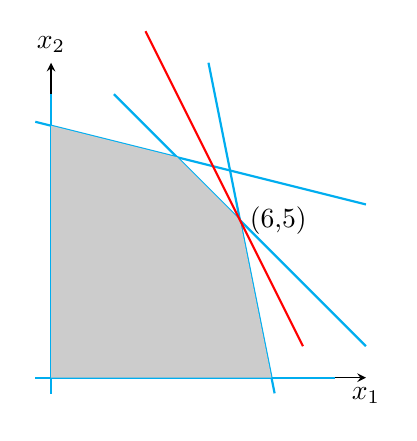
\begin{tikzpicture}[xscale=0.4,yscale=0.4]
            % draw the axis
            \draw[eaxis] (-0.5,0) -- (10,0) node[below] {$x_1$};
            \draw[eaxis] (0,-0.5) -- (0, 10) node[above] {$x_2$};
            % draw the function (piecewise)
            \draw[elegant,domain=-0.5:10] plot(\x,{-\x/4+8});
            \draw[elegant,domain=2:10] plot(\x,{-\x+11});
            \draw[elegant,domain=5:7.1] plot(\x,{-5*\x+35});
            \draw[elegant,domain=-0.5:9] plot(\x,0);
            \draw[elegant,domain=-0.5:9] plot(0,\x);
            \fill[gray!40] (0,0) -- (7,0) -- (6,5) -- (4,7) -- (0,8) -- (0,0);

            \draw[elegant,red,domain=3:8] plot(\x,{-2*\x+17});

            \node at (6,5) [right] {(6,5)};
        \end{tikzpicture}
      }
      \end{center}
      得到$\max z = 17$;
      \item 
      $x_2 = -x_1 + z$\\
      画图:
      \begin{center}
      \resizebox{0.6\linewidth}{!}{
        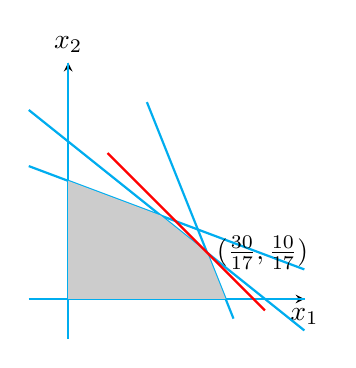
\begin{tikzpicture}
            % draw the axis
            \draw[eaxis] (-0.5,0) -- (3,0) node[below] {$x_1$};
            \draw[eaxis] (0,-0.5) -- (0, 3) node[above] {$x_2$};
            % draw the function (piecewise)
            \draw[elegant,domain=-0.5:3] plot(\x,{-4*\x/5+2});
            \draw[elegant,domain=1:2.1] plot(\x,{-5*\x/2+5});
            \draw[elegant,domain=-0.5:3] plot(\x,{-3*\x/8+3/2});
            \draw[elegant,domain=-0.5:3] plot(\x,0);
            \draw[elegant,domain=-0.5:3] plot(0,\x);
            \fill[gray!40] (0,0) -- (2,0) -- (30/17,10/17) -- (20/17,18/17) -- (0,3/2) -- (0,0);

            \draw[elegant,red,domain=0.5:2.5] plot(\x,{-\x+40/17});

            \node at (30/17,10/17) [right] {($\frac{30}{17},\frac{10}{17}$)};
        \end{tikzpicture}
      }
      \end{center}
      得到$\max z = \frac{40}{17}$;
      \item 
      $x_2 = -x_1 + \frac{z}{2}$\\
      画图:
      \begin{center}
      \resizebox{0.6\linewidth}{!}{
        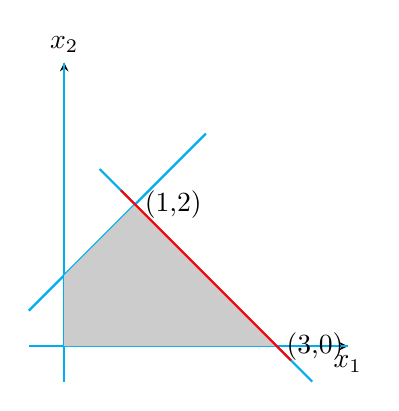
\begin{tikzpicture}[xscale=0.9,yscale=0.9]
            % draw the axis
            \draw[eaxis] (-0.5,0) -- (4,0) node[below] {$x_1$};
            \draw[eaxis] (0,-0.5) -- (0, 4) node[above] {$x_2$};
            % draw the function (piecewise)
            \draw[elegant,domain=-0.5:2] plot(\x,{\x+1});
            \draw[elegant,domain= 0.5:3.5] plot(\x,{-\x+3});
            \draw[elegant,domain=-0.5:4] plot(\x,0);
            \draw[elegant,domain=-0.5:4] plot(0,\x);
            \fill[gray!40] (0,0) -- (3,0) -- (1,2) -- (0,1) -- (0,0);

            \draw[elegant,red,domain=0.8:3.2] plot(\x,{-\x+3});

            \node at (3,0) [right] {(3,0)};
            \node at (1,2) [right] {(1,2)};
        \end{tikzpicture}
      }
      \end{center}
      得到$\max \frac{z}{2} = 3$,即$\max z = 6$;
      \item 
      $x_2 = -x_1 + z$\\
      画图:
      \begin{center}
      \resizebox{0.6\linewidth}{!}{
        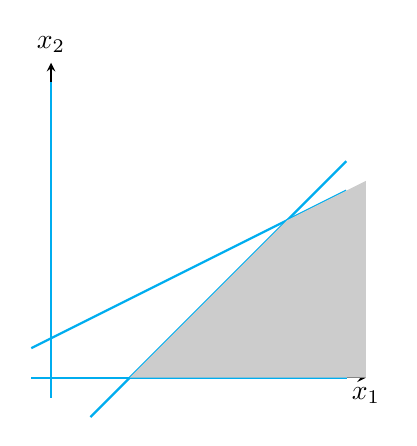
\begin{tikzpicture}[xscale=0.5,yscale=0.5]
            % draw the axis
            \draw[eaxis] (-0.5,0) -- (8,0) node[below] {$x_1$};
            \draw[eaxis] (0,-0.5) -- (0, 8) node[above] {$x_2$};
            % draw the function (piecewise)
            \draw[elegant,domain=-0.5:7.5] plot(\x,{\x/2+1});
            \draw[elegant,domain=1:7.5] plot(\x,{\x-2});
            \draw[elegant,domain=-0.5:7.5] plot(\x,0);
            \draw[elegant,domain=-0.5:7.5] plot(0,\x);
            
            \fill[gray!40] (8,0) -- (2,0) -- (6,4) -- (8,5) -- (8,0);

            % \draw[elegant,red,domain=1:2.5] plot(\x,{-\x+2});
            % \node[circle,draw=black, fill=gray!40, inner sep=0pt,minimum size=2pt] (b) at (2,0) {};
            % \node at (2,0) [right] {(2,0)};
        \end{tikzpicture}
      }
      \end{center}
      得到$\max z = +\infty$;
   \end{enumerate}
\end{solution}
  \item 已知$n$是正整数,$d_1=1,d_2,d_3,\ldots,d_r=n$是$n$的除数,即$d_i\mid n,i=1,2,\ldots,r$,
试证:$\sum_{d_i}\phi(d_i)=n$。
  \begin{solution}
   \begin{enumerate}
      \item 任意两个拉丁方组合的结果:
      \begin{align*}&
         \left[\begin{matrix}
             (1,3)&(3,1)&(2,4)&(4,2)\\
             (3,2)&(1,4)&(4,1)&(2,3)\\
             (2,1)&(4,3)&(1,2)&(3,4)\\
             (4,4)&(2,2)&(3,3)&(1,1)
         \end{matrix}\right],
         \left[\begin{matrix}
             (3,2)&(1,4)&(4,1)&(2,3)\\
             (2,1)&(4,3)&(1,2)&(3,4)\\
             (1,3)&(3,1)&(2,4)&(4,2)\\
             (4,4)&(2,2)&(3,3)&(1,1)
         \end{matrix}\right],\\&
         \left[\begin{matrix}
            (1,2)&(3,4)&(2,1)&(4,3)\\
            (3,1)&(1,3)&(4,2)&(2,4)\\
            (2,3)&(4,1)&(1,4)&(3,2)\\
            (4,4)&(2,2)&(3,3)&(1,1)
        \end{matrix}\right].
     \end{align*}
     每个组合中均不存在相同元素,即两两正交。又n阶拉丁方的正交族元素数
     至多为n-1,所以上述3个4阶的拉丁方构成正交族;
     \item 上述3个5阶拉丁方任意两个组合均不存在相同元素,即两两正交。
     但是存在另一个拉丁方:
     \begin{align*}
      \left[\begin{matrix}
          1&2&3&4&5\\
          4&5&1&2&3\\
          2&3&4&5&1\\
          5&1&2&3&4\\
          3&4&5&1&2\\
         \end{matrix}\right]
      \end{align*}
      与上述3个5阶拉丁方均正交。即5阶正交拉丁方族的大小应当为4,上述3个个5阶拉丁方不构成
      正交拉丁方族。
   \end{enumerate}
\end{solution}
  \item 有$n$个不同的整数,从中取出两组数来,要求第1组的最小数大于另一组的最大数。
  \begin{proof}
    将单位正方形沿两个对边的中点分成4个边长为$\frac{1}{2}$的小正方形。根据容斥原理,将9个点放在4个小正方形中,
    其中必然至少存在一个小正方形中包含有3个点。这三个点构成的三角形面积最大为
    $\frac{1}{2}\cdot\frac{1}{2}\cdot\frac{1}{2}=\frac{1}{8}$,得证。
\end{proof}

\end{enumerate}


\end{document}